%%%%%%%%%%%%%%%%%%%%%%%%%%%%%%%%%%%%%%%%%%%%%%%%%%%%%%%%%%%%%%%%%%%%%%%%%%%%%%%%
\section{What is Snakemake?}

%%%%%%%%%%%%%%%%%%%%%%%%%%%%%%%%%%%%%%%%%%%%%%%%%%%%%%%%%%%%%%%%%%%%%%%%%%%%%%%%
\begin{frame}
	\frametitle{Outline}
	\begin{columns}[t]
		\begin{column}{.5\textwidth}
			\tableofcontents[sections={1-7},currentsection]
		\end{column}
		\begin{column}{.5\textwidth}
			\tableofcontents[sections={8-15},currentsection]
		\end{column}
	\end{columns}
\end{frame}

%%%%%%%%%%%%%%%%%%%%%%%%%%%%%%%%%%%%%%%%%%%%%%%%%%%%%%%%%%%%%%%%%%%%%%%%%%%%%%%%
\begin{frame}
	\frametitle{What is this about?}
	\begin{question}[Questions]
		\begin{itemize}
			\item Why \Snakemake?
			\item Why not "Something Else"?
			\item Why Clusters?
		\end{itemize}
	\end{question}
	\begin{docs}[Objectives]
		\begin{enumerate}
			\item Introduction to \Snakemake Usage (in-depth will follow)
			\item Get an Mini-Overview about Workflow Systems
		\end{enumerate}
	\end{docs}
\end{frame}

%%%%%%%%%%%%%%%%%%%%%%%%%%%%%%%%%%%%%%%%%%%%%%%%%%%%%%%%%%%%%%%%%%%%%%%%%%%%%%%%
\begin{frame}[fragile]
	\frametitle{How does \Snakemake work?}
	\begin{columns}[t]
		\begin{column}{.5\textwidth}
			\begin{itemize}[<+->]
			  \item Snakemake is triggered on the command line:
			  \begin{lstlisting}[language=Bash, style=Shell]
$ snakemake [<arguments>]
			  \end{lstlisting} 
			  \end{itemize}
			  \item you will fill in the parameters of your workflow (in a file)
			  \item Snakemake will spawn your jobs on the cluster
		\end{column}
		\begin{column}{.5\textwidth}
			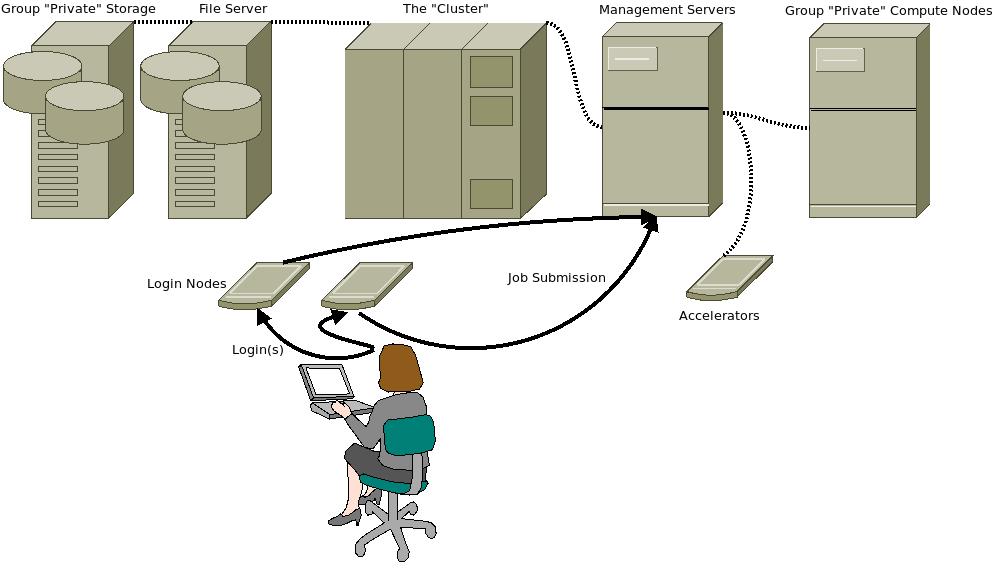
\includegraphics[width=0.95\textwidth]{misc/cluster_scheme.png}
		\end{column}
	\end{columns}
	